\documentclass[12pt,a4paper]{report}

\usepackage[utf8]{inputenc}
\usepackage{amsmath}
\usepackage{amsfonts}
\usepackage{amssymb}
%\usepackage[pdftex,
	%pdfauthor={Quentin Van de Kadsye et Jérôme Tanghe},
	%pdftitle={Projet encadré : #currentmood},
	%pdfsubject={Analyse de l'humeur de tweets},
	%pdfkeywords={twitter currentmood pje pje2},
	%pdfproducer={LaTeX},
	%pdfcreator={PDFLaTeX}]{hyperref}
\usepackage{hyperref}
\usepackage{graphicx}
\usepackage{titlesec}
\usepackage{booktabs}
\usepackage{eurosym}
\usepackage[justification=centering,font={small,sf},labelfont=bf]{caption}
\usepackage[table]{xcolor}
\usepackage[francais]{babel}
\usepackage[left=2cm,right=2cm,top=2cm,bottom=2cm]{geometry}

\newcommand{\CMName}{\#currentmood}

% Personnalisation des chapitres
\titleformat{\chapter}[hang]
{\fontfamily{cmss}\bfseries\huge}{\Roman{chapter} --- }{0cm}{%
	\vspace{1ex}
}

% Personnalisation des sections
\titleformat{\section}[hang]
{\bfseries\LARGE}{\arabic{section} --- }{0cm}{%
	\vspace{1ex}
}

% Personnalisation des sous-sections
\titleformat{\subsection}[hang]
{\bfseries\large}{}{0cm}{%
	\vspace{0ex}
}

% Personnalisation des tableaux
\arrayrulecolor{lightgray}

\title{PJE\\\CMName}
\author{Quentin Van de Kadsye \and Jérôme Tanghe}
\date{Mardi 15 décembre 2015}

\setlength{\parskip}{\baselineskip}

\begin{document}
%\maketitle
\newgeometry{left=0cm,right=0cm,top=5cm,bottom=5cm}
\begin{titlepage}
	\centering
	{%
		\fontfamily{cmss}
		\Huge

		\textbf{PJE}

		\CMName%

		\vfill

		
\includegraphics[width=0.25\textwidth]{img/TwitterLogo.eps}

		\Large
		\vfill

		Quentin Van de Kadsye
		\hspace{2cm}
		Jérôme Tanghe

		\vfill
		Université Lille 1
	}
\end{titlepage}

\newgeometry{left=2cm,right=2cm,top=2cm,bottom=2cm}

\setcounter{tocdepth}{1}
\tableofcontents

% -----------------------------------------------------------------------------

\chapter{Le projet}

Il est parfois intéressant pour les entreprises de connaître l'humeur générale
des internautes concernant un sujet donné. Twitter étant une plateforme où l'on peut
s'exprimer librement, c'est donc un emplacement de choix pour récolter ce type
d'information. Se pose alors le problème suivant: comment connaître rapidement
l'humeur des personnes sur un sujet donné?

Nommé selon le hashtag du même nom, \textbf{\CMName} est un programme tentant de
répondre à ce besoin. Écrit en Java, il permet d'estimer l'humeur d'un ou
plusieurs messages publiés sur Twitter (\textit{Tweet}), à l'aide d'une des trois méthodes proposées:

\begin{itemize}
	\item
		\textbf{Mots-clés:} utilise une liste de mots prédéfinis dans des
		fichiers pour déterminer l'humeur du Tweet.
	\item
		\textbf{KNN:} évalue l'humeur d'un Tweet en fonction de l'humeur de $k$
		autres Tweets, en recherchant dans une base de données de Tweets dont on
		connaît déjà l'humeur ceux qui contiennent les mêmes mots.
	\item
		\textbf{Classification bayésienne:} évalue la probabilité d'humeur d'un
		Tweet en calculant la probabilité que les mots qu'il contient
		appartiennent à cette humeur à partir de la base de données.
\end{itemize}

Le code source du logiciel est disponible sur GitHub:
\texttt{\href{http://github.com/Deuchnord/currentmood}{github.com/Deuchnord/currentmood}}.

\begin{figure}
	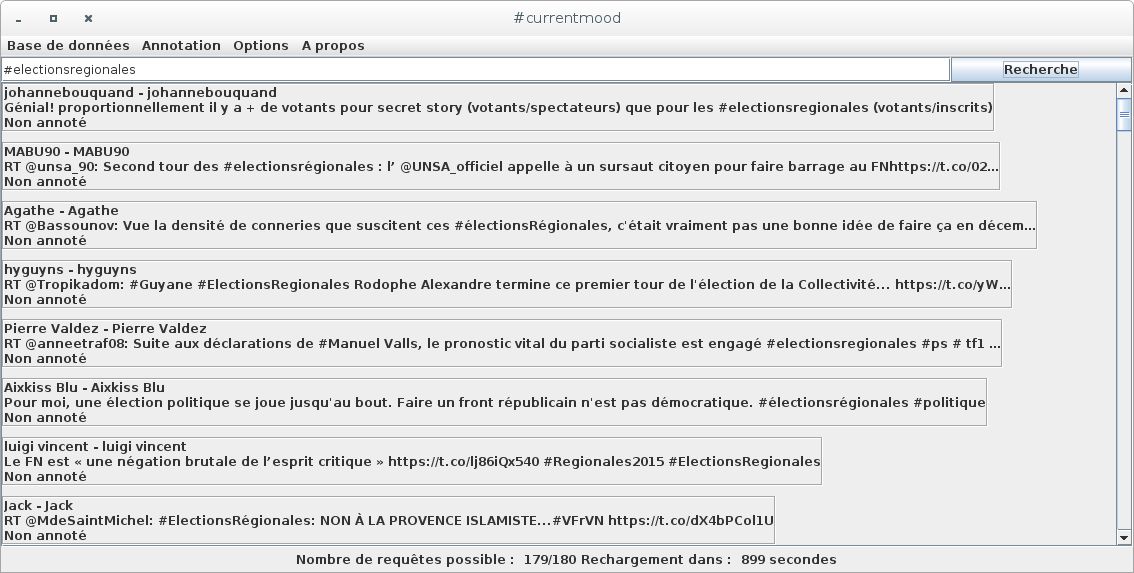
\includegraphics[width=\textwidth]{img/capture-currentmood-ui.png}
	\caption{Interface utilisateur générale de \CMName}
\label{cm_ui}
\end{figure}


% -----------------------------------------------------------------------------
\chapter{L'interface de \CMName}
Ayant fait le choix de développer l'application grâce au langage Java, nous
avons choisi d'utiliser la bibliothèque graphique Swing, avec laquelle nous
avons le plus d’expérience.

\section{Utilisation d'un serveur proxy}
Si, pour une raison quelconque, vous devez utiliser un serveur proxy, alors il
faut préciser les paramètres proxy à l'application. Pour ce faire, ouvrez le
menu \textit{Options} et choisissez \textit{Paramètres proxy}
(figure~\ref{capture_menuproxy}).

\begin{figure}
	\centering
	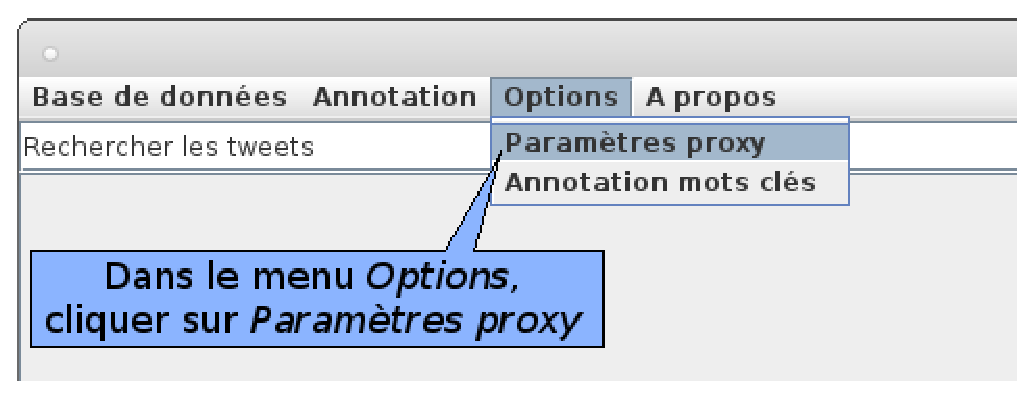
\includegraphics[width=0.75\textwidth]{img/capture_menuproxy.eps}
	\caption{Accès aux paramètres Proxy}
\label{capture_menuproxy}
\end{figure}

La fenêtre de configuration du Proxy s'affiche alors
(figure~\ref{capture_fenproxy} page~\pageref{capture_fenproxy}), il suffit de
remplir les paramètres nécessaires et de valider. Nous avons également
implémenté un bouton afin de régler en un clic les paramètres pour le Proxy de
l'Université de Lille 1: il suffit de cliquer dessus pour remplir les champs
adéquats, et enfin de valider.

\begin{figure}
	\centering
	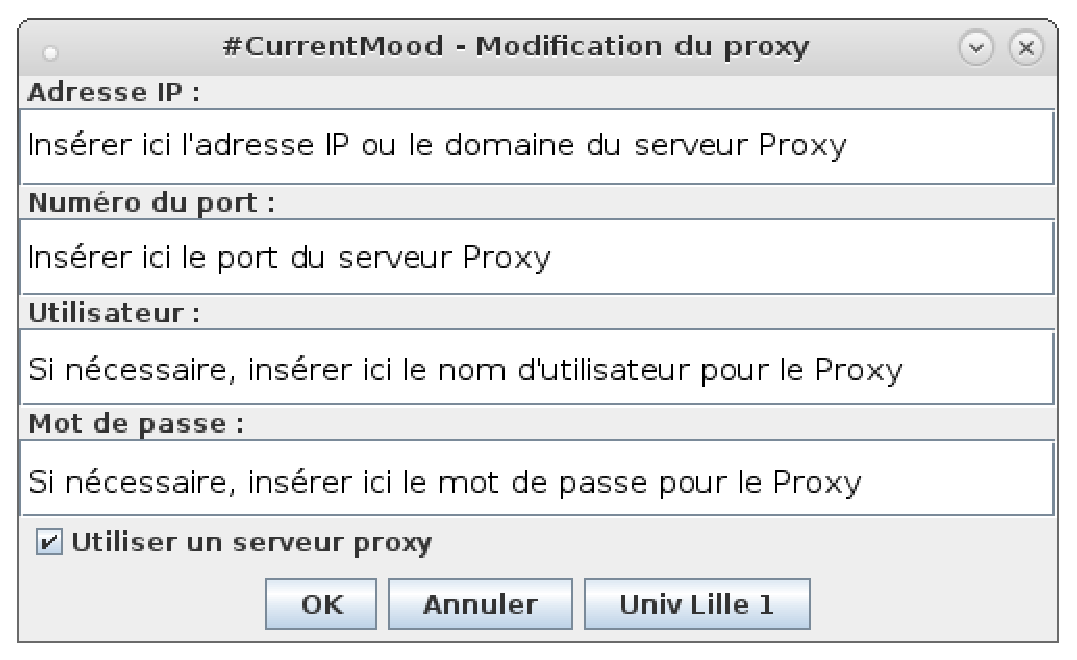
\includegraphics[width=0.75\textwidth]{img/capture_fenproxy.eps}
	\caption{Fenêtre de configuration du Proxy}
\label{capture_fenproxy}
\end{figure}

\newpage
\section{Effectuer une recherche  et annoter manuellement}
Pour rechercher un Tweet, il suffit de taper ses mots-clés dans la zone de
saisie en haut de la fenêtre et de cliquer sur le bouton \textit{Rechercher}
(figure~\ref{capture_rechercherTweet}).
On peut alors annoter un Tweet à la main \textit{via} son menu contextuel
(figure~\ref{capture_annoterTweet} page~\pageref{capture_annoterTweet}).

\begin{figure}
	\centering
	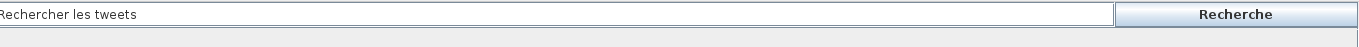
\includegraphics[width=\textwidth]{img/chercheruntweet.png}
	\caption{Zone de recherche de \CMName}
\label{capture_rechercherTweet}
\end{figure}


\begin{figure}
	\centering
	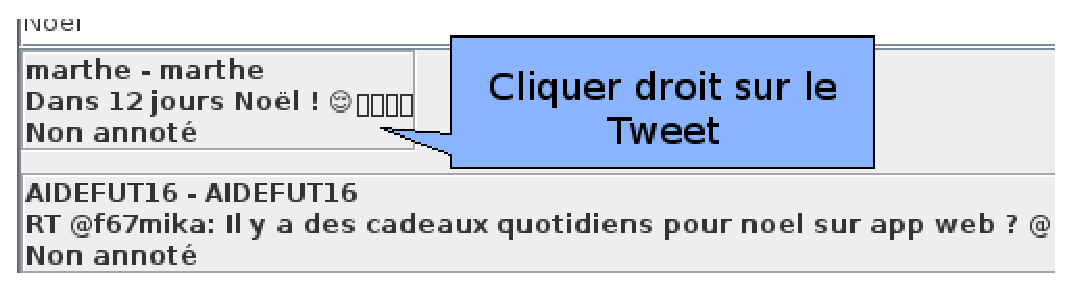
\includegraphics[width=\textwidth]{img/capture_annotertweet1.eps}
	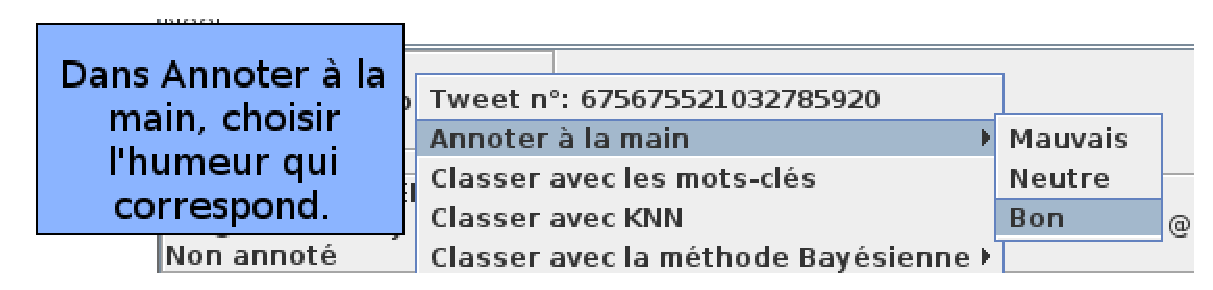
\includegraphics[width=\textwidth]{img/capture_annotertweet2.eps}
	\caption{Annoter un Tweet}
\label{capture_annoterTweet}
\end{figure}

Ce même menu permet par ailleurs d'annoter un Tweet automatiquement par les
méthodes des mots-clés, KNN ou bayésienne.

\section{Annoter automatiquement}
Pour annoter tous les Tweets automatiquement selon une des méthodes
implémentées, il faut, si la méthode l'exige, charger la base de données
(figure~\ref{capture_ouvrir_base_de_donnees}). Une fenêtre s'ouvrira pour
montrer la répartition des humeurs (figure~\ref{capture_repartition_Tweetsv6}).

\begin{figure}
	\centering
	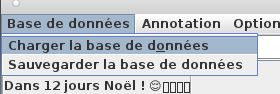
\includegraphics[width=0.5\textwidth]{img/chargerbdd.png}
	\caption{Menu d'ouverture de la base de données}
\label{capture_ouvrir_base_de_donnees}
\end{figure}

\begin{figure}
	\centering
	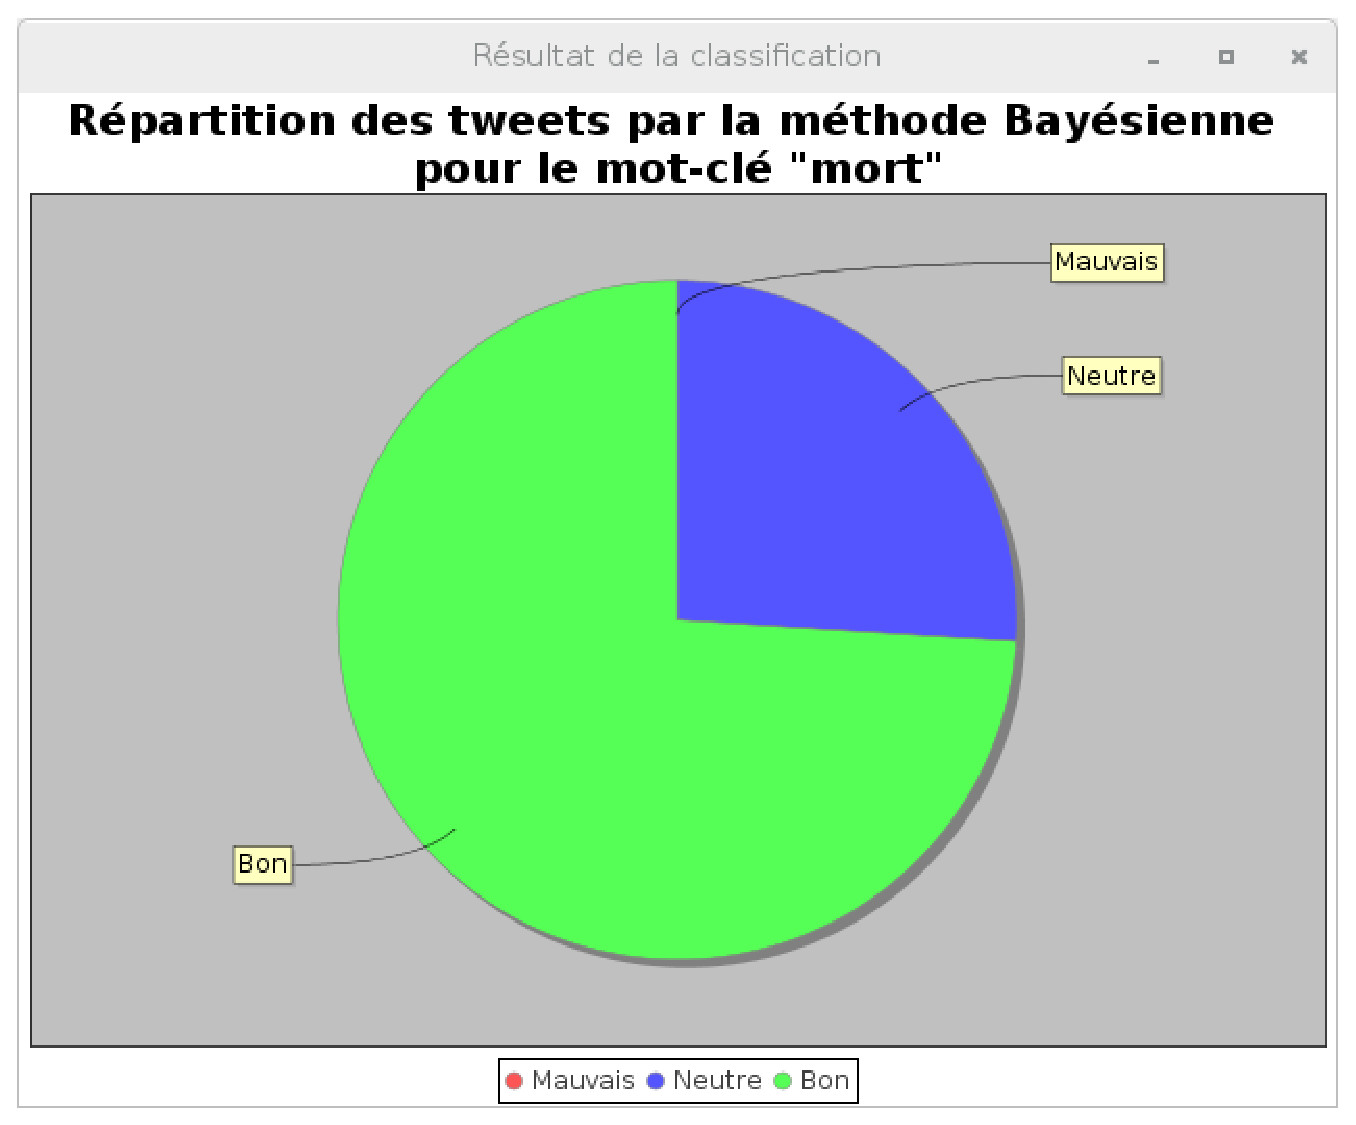
\includegraphics[width=\textwidth]{img/resultats_classification_tweetsv6.eps}
	\caption{Fenêtre affichant la répartition des Tweets dans une base de
	données}
\label{capture_repartition_Tweetsv6}
\end{figure}


Pour annoter un Tweet automatiquement, deux stratégies sont possibles.
La première consiste à annoter automatiquement un seul Tweet par le biais de son
menu contextuel (figure~\ref{capture_annoterTweet}
page~\pageref{capture_annoterTweet}), la deuxième à annoter la
totalité des Tweets correspondant à une recherche, \textit{via} le menu
\textit{Annoter}.

% -----------------------------------------------------------------------------

\chapter{API Twitter et gestion des Tweets}

\section{La classe \texttt{CMTwitter}}

Afin de communiquer avec l'API de Twitter, nous avons utilisé la librairie
\textbf{Twitter4J}\footnote{\href{http://twitter4j.org}{twitter4j.org}} qui
propose les fonctionnalités dont nous avons besoin pour mener à bien le projet.
Pour faciliter son implémentation, nous avons également créé une classe,
\texttt{CMTwitter}, s'interfaçant entre notre application et Twitter4J, comme le
montre la figure~\ref{uml_cmtwitter} (page~\pageref{uml_cmtwitter}).

\begin{figure}%[h]
	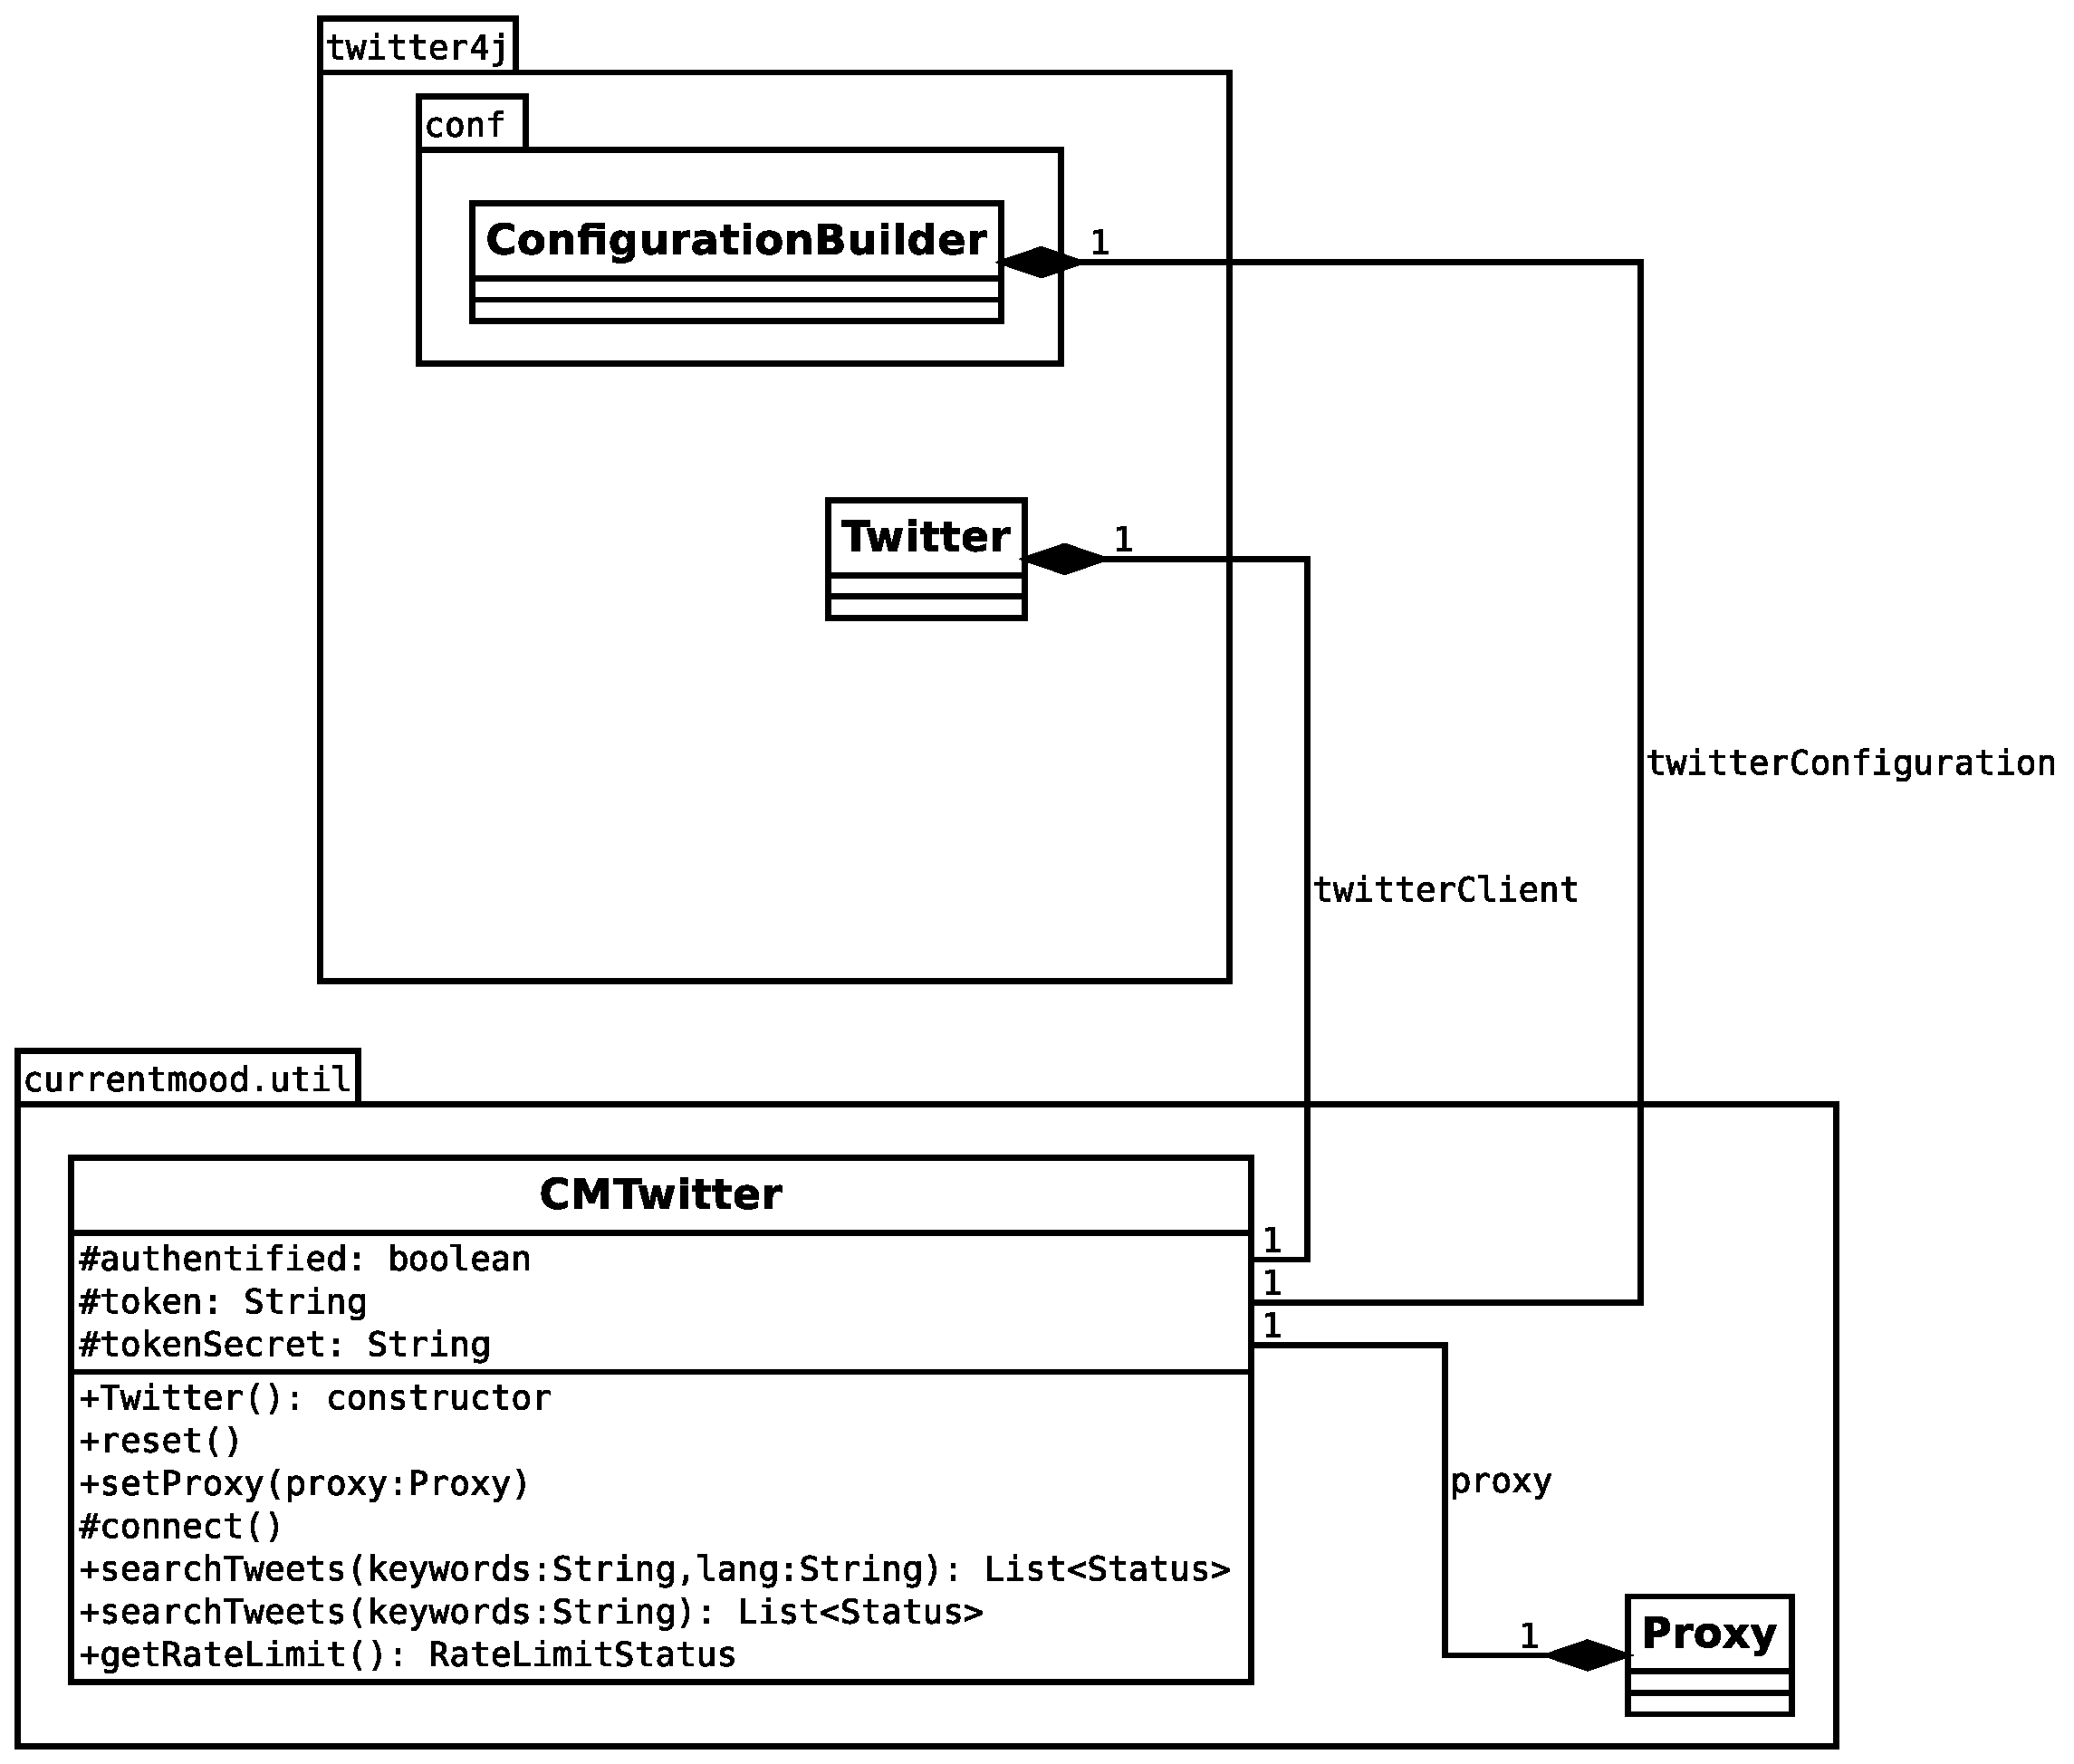
\includegraphics[width=\textwidth]{img/uml_cmtwitter.eps}
	\caption{Diagramme de classe montrant comment nous interfaçons Twitter4J}
\label{uml_cmtwitter}
\end{figure}

Cela nous permet d'utiliser l'API de Twitter à l'aide de trois méthodes
principales seulement au lieu d'une dizaine:

\begin{itemize}
	\item
		\texttt{setProxy()} afin de donner les paramètres proxy à Twitter4J;
	\item
		\texttt{connect()} afin d'établir la connexion avec l'API de Twitter;
	\item
		\texttt{searchTweets()} afin d'utiliser la fonction de recherche de
		l'API de Twitter.
\end{itemize}

La méthode \texttt{reset()}, quant à elle, est utilisée par les méthodes
précédentes afin de permettre d'effectuer plusieurs requêtes. En effet, nous
avons pu remarquer que l'objet \texttt{ConfigurationBuilder} périme après chaque
requête, nous obligeant à le recréer avant d'effectuer une nouvelle requête.

L'utilisation de cette classe s'effectue en trois étapes principales.

Tout d'abord, on configure si nécessaire les paramètres proxy à l'aide de la
méthode \texttt{setProxy()}. Cette dernière donne lesdits paramètres à l'objet
\texttt{ConfigurationBuilder}.

Ensuite, on appelle la méthode \texttt{connect()} qui utilise l'objet
\texttt{ConfigurationBuilder} pour obtenir une instance de \texttt{Twitter}.

C'est cette instance qui est ensuite utilisée par \texttt{searchTweets()} qui
instancie un objet de Twitter4J permettant d'obtenir des Tweets correspondant
à la recherche. Cette méthode retourne une liste d'objets \texttt{Status}
provenant de la librairie Twitter4J.

\newpage
\section{La classe \texttt{Tweet}}

Nous nous sommes rapidement rendus compte que Twitter4J ne proposait aucune
classe implémentant l'interface \texttt{Status} que nous devons manipuler. De
plus, les objets que nous en obtenons contient de nombreuses informations qui ne
nous sont pas utiles, tandis que d'autres nous étaient nécessaires mais
n'y étaient pas présents.

Nous avons donc créé une classe indépendante de Twitter4J, \texttt{Tweet}, qui
réponde à ce besoin (figure~\ref{uml_Tweet}). Elle est utilisée dans toute l'application afin de contenir
chaque Tweet.

\begin{figure}
	\centering
	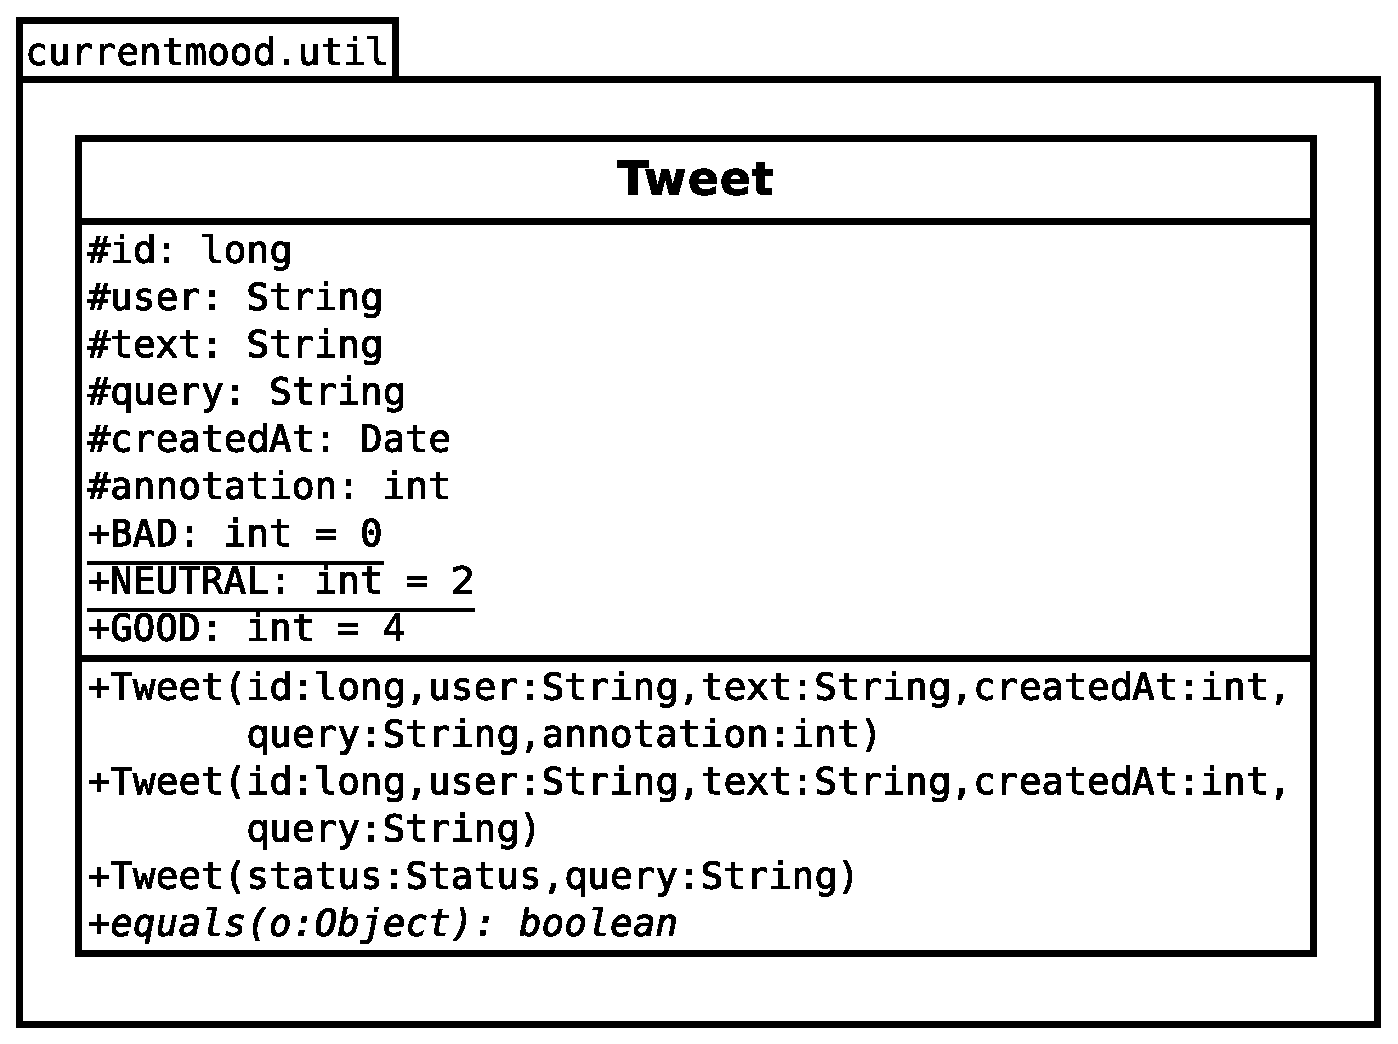
\includegraphics[width=9cm]{img/uml_tweet.eps}
	\caption{La classe \texttt{Tweet}}
\label{uml_Tweet}
\end{figure}

Cette classe est surtout composée d'accesseurs permettant d'accéder à chaque
propriété du Tweet. Ses deux premiers constructeurs permettent de créer un objet
à partir de données déjà connues (typiquement lors de l'ouverture d'un fichier
CSV), tandis que le troisième permet d'obtenir un objet \texttt{Tweet} à partir
d'un objet \texttt{Status} généré par Twitter4J.

Nous avons également surchargé la méthode \texttt{equals()} de la super-classe
\texttt{Object} afin de permettre la comparaison de l'objet courant avec un
autre objet \texttt{Tweet}. Cela nous sera nécessaire pour certaines actions par
la suite.

% -----------------------------------------------------------------------------
\chapter{La base d'apprentissage}

\section{Le nettoyage des Tweets}

L'annotation automatique se basant sur une base d'apprentissage construite
manuellement, il est primordial d'avoir une base de données saine pour éviter
les erreurs d'interprétation. Cela passe par un nettoyage des Tweets afin de
limiter le «~bruit~».

Lors de la sauvegarde des Tweets annotés manuellement dans un fichier CSV, nous
passons par une étape consistant à supprimer tout ce qui peut gêner
l'interprétation du Tweet ou la lecture du fichier CSV.\@

Ainsi, nous supprimons:

\begin{itemize}
	\item
		Les retours à la ligne (pour respecter le format CSV)
	\item
		Les smileys \texttt{:)}, \texttt{:(}, \texttt{:D}, \texttt{:')},
		\texttt{:'(} et \texttt{:'D}
	\item
		Les liens hypertextes
	\item
		Les \texttt{@usernames}
	\item
		Les hashtags
	\item
		La ponctuation
	\item
		Les symboles monnétaires principaux (\euro, \$, £)
	\item
		Les pourcentages
\end{itemize}

Une fois ce nettoyage effectué, nous pouvons alors utiliser cette base de Tweets
pour annoter automatiquement d'autres Tweets selon quatre méthodes qui seront
traitées dans la
partie~\ref{chapter-classifications}~(page~\pageref{chapter-classifications}).
Ce nettoyage permet également d'enregistrer les Tweets dans un fichier CSV sans
casser son format (en supprimant notamment les retours à la ligne et les
virgules).

\section{Le fichier CSV}

Pour gérer la base de données, il a été décidé de sauvegarder les messages
annotés dans un fichier CSV\footnote{\textit{Comma-separated values}}. Ce type
de fichier a pour principal avantage d'être relativement léger et facile à lire
par programmation.

Les données à sauvegarder étant globalement celles contenues dans les objets
\texttt{Tweet}, l'ordre de sauvegarde sera donc le suivant:

\begin{enumerate}
	\item
		Le numéro d'identification du Tweet
	\item
		Le nom de l'auteur du Tweet
	\item
		Le contenu du Tweet
	\item
		La date et l'heure du Tweet, sous la forme d'un
		\textit{timestamp}\footnote{Nombre de secondes depuis le 
		1\ier{} janvier 1970, 0 h 00 min 00 s GMT}. S'il est nul, il est
		ignoré.
	\item
		La recherche qui a permis de trouver le Tweet
	\item
		L'annotation du Tweet
\end{enumerate}

L'annotation du Tweet est enregistrée sous la forme d'un nombre dont la valeur
est précisé par le tableau~\ref{tableau-valeurs-annotation}.

\begin{table}[h]
	\centering
	\begin{tabular}{c c}
		\textbf{Valeur de l'annotation}	& \textbf{Humeur du Tweet}\\
		\midrule
		$0$				& Mauvais\\
		\midrule
		$2$				& Neutre\\
		\midrule
		$4$				& Bon
	\end{tabular}
	\caption{Valeur de l'annotation selon l'humeur du Tweet}
\label{tableau-valeurs-annotation}
\end{table}

% -----------------------------------------------------------------------------
\chapter{Classification automatique des Tweets}
\label{chapter-classifications}

\section{Classification par mots-clés}
La classification par mots-clés est la plus simple des méthodes de
classification. Elle consiste à se baser sur une liste de mots définis dans un
fichier pour déterminer l'humeur d'un Tweet.

Sa stratégie est des plus simples: pour un Tweet donné, on recherche
chacun de ses mots dans un dictionnaire définissant des mots positifs et des
mots négatifs. Leur nombre respectifs déterminera alors l'humeur du Tweet. Par
exemple, un Tweet contenant 3 mots considérés positifs et 5 mots considérés
négatifs sera annoté négatif. Un Tweet qui contiendrait un même nombre de mots
positifs et négatifs est considéré comme étant neutre.

\subsection{Annoter par mots-clés dans \CMName}
Avant toute chose, il est nécessaire de charger le dictionnaire de mots positifs
et de mots négatifs. Pour ce faire, dans le menu \textit{Options}, cliquez sur
\textit{Annotation mots clés}:

\begin{figure}[h]
	\centering
	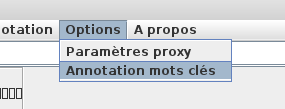
\includegraphics[width=0.5\textwidth]{img/capture_menumotcle.png}
\end{figure}

Le programme demande alors de sélectionner le fichier contenant les mots
positifs, puis les mots négatifs (figure~\ref{ouvrir_dictionnaire}
page~\pageref{ouvrir_dictionnaire}).

\begin{figure}[h]
	\centering
	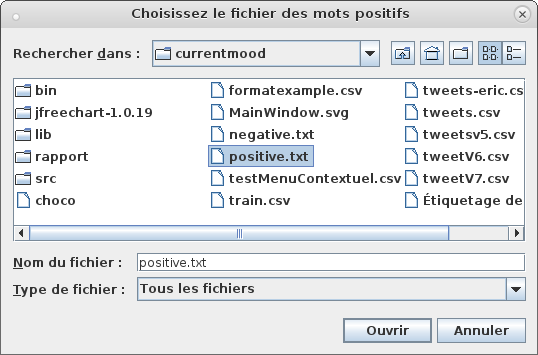
\includegraphics[width=0.4\textwidth]{img/capture_ouvrir-mots-positifs.png}
	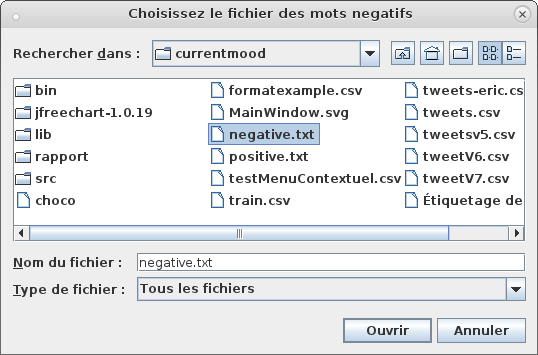
\includegraphics[width=0.4\textwidth]{img/capture_ouvrir-mots-negatifs.png}
	\caption{Ouverture du dictionnaire de mots positifs et négatifs}
\label{ouvrir_dictionnaire}
\end{figure}

\newpage
\subsection{Résultats de la classification}
Cet algorithme s'est révélé peu efficace du fait qu'il se contente de réduire
une phrase complète à de simples mots auquel il donne un sens \textit{a priori}.
Il ne prend de ce fait pas compte du sens général du Tweet. Prenons par exemple
le Tweet suivant :

\begin{quote}
	\textit{Génial, ma banque m'a refusé mon crédit…}
\end{quote}

On remarque bien que ce Tweet est plutôt négatif. Cependant, la présence du mot
\textit{génial} peut influencer la classification finale, ce qui peut déboucher,
ici, à un faux positif.

Cet algorithme nécessite également que le dictionnaire utilisé contienne
suffisamment de mots: en effet, un dictionnaire pas assez fourni signifierait
que de nombreux Tweets seraient soit mal annotés (en raison de la présence
d'autres mots connus) ou annotés neutre.

Il est à ce titre intéressant de remarquer que le terme \textit{neutre} n'a ici
pas le même sens que dans les autres classifications. En effet, ici,
\textit{neutre} signifie que le Tweet n'a pas pu être annoté soit parce qu'il ne
contenait aucun mot connu du dictionnaire, soit parce qu'il contenait autant de
mots positifs que de mots négatifs.qu'il contenait autant de mots positifs que
de mots négatifs.

\section{Classification par la méthode KNN}
La méthode des $k$ plus proches voisins, ou KNN\footnote{$k$-nearest neighbor},
est une méthode consistant à exploiter la base d'apprentissage en comptant le
nombre de mots en commun entre un Tweet à annoter et chaque Tweet de la base.

L'humeur du Tweet est alors déterminée selon l'humeur des $k$ Tweets
avec lesquels il a le plus de mots en commun.

Pour ce faire, l'algorithme calcule la distance entre le Tweet à annoter (que
l'on nommera $A$ par la suite) et chaque Tweet de la base de données
en conservant les $k$ Tweets les plus proches ($k$ étant un nombre
choisi par l'utilisateur). Il en déduit alors l'humeur du Tweet $A$ en comparant
simplement le nombre de Tweets positifs, neutres et négatifs parmi les $k$ plus
proches.

L'intérêt d'utiliser un nombre $k$ est que l'on utilise alors un nombre réduit
de Tweets parmi ceux les plus proches, ce qui permet d'influer sur la précision
de l'algorithme.

\subsection{Observations}
De part sa conception, cette méthode est plutôt sensible à la répartition des
Tweets enregistrés dans la base de données. En effet, si une des humeurs y est
majoritaire par rapport aux autres, elle influencera grandement le résultat.

Ainsi, nous avons pu constater qu'avec une base de données contenant environ
80\% de Tweets positifs, quasimment tous les Tweets annotés par la méthode KNN
seront considérés positifs.

Pour que la méthode soit efficace, nous avons fait des tests avec plusieurs
valeurs de $k$, et nous avons pu remarquer que, pour une base de $n$ Tweets:

\begin{itemize}
	\item si $k=1$, la méthode est peu efficace, car elle n'utilise que
		\textit{le} plus proche voisin. L'humeur de ce voisin est donc
		toujours le résultat, qui peut être faux;
	\item si $k=n$, on utilise toute la base de données et cela revient presque
		à utiliser la méthode par mots-clés, puisque l'on prend la majorité de
		tous les Tweets présents dans la base;
	\item si $1 < k < n$, on utilisera un nombre plus ou moins conséquents de
		voisins, ce qui permet d'avoir une plus grande variété pour déterminer
		l'humeur du Tweet.
\end{itemize}

\section{Classification par la méthode bayésienne}
\label{classification_bayesienne}
La méthode de classification bayésienne est une méthode de classification
probabiliste. Dans le cas de notre application, elle servira à déterminer la
probabilité qu'un Tweet appartienne à l'une des classes établies précédemment,
c'est-à-dire : mauvais, neutre ou bon.

Afin de pouvoir évaluer un Tweet, il faut d'abord calculer P(c) : la probabilité
d'appartenance à une classe (P(M), P(N), P(B)).
Un Tweet étant un ensemble de mots, il a fallu déterminer l'appartenance d'un
mot à une classe. Pour cela il a été nécessaire de répertorier la classe de
chaque mot de chaque Tweet se trouvant dans la base de données pour chaque
classe.

Ensuite avec une formule mathématique, on calcule la probabilité que le Tweet
appartienne à la classe mauvais, neutre ou bon.

\begin{itemize}
	\item
		La méthode par présence ou fréquence en se servant de tous les mots et
		par unigramme.
	\item
		La méthode par présence ou fréquence en servant de tous les mots et par
		bigramme.
	\item
		La méthode par présence ou fréquence en enlevant tous les mots de moins
		de trois lettres (à, de…) et par unigramme.
	\item
		La méthode par présence ou fréquence en enlevant tous les mots de moins
		de trois lettres (à, de…) et par bigramme.
\end{itemize}

\subsection{Que sont les unigrammes et les bigrammes?}
Les unigrammes et les bigrammes sont en réalité des ensembles de mots, un
unigramme est donc un ensemble composé d'un seul et unique mot. Un bigramme est
un ensemble composé de deux mots, Ainsi « Chef-d'œuvre » peut être considéré
comme un bigramme.

Le fait d'enlever les mots de moins de trois lettres, comme les prépositions,
permet d'avoir des probabilités plus fines: en effet, les probabilités étant
calculées en fonction de la probabilité d'appartenance à une classe pour chaque
mot, et qu'il est difficile d'attribuer une classe à un mot comme une
préposition, le résultat peut être faussé, comme le montrent les
figures~\ref{bayes_tous_les_mots} et~\ref{bayes_pas_tous_les_mots}.

\begin{figure}
	\centering
	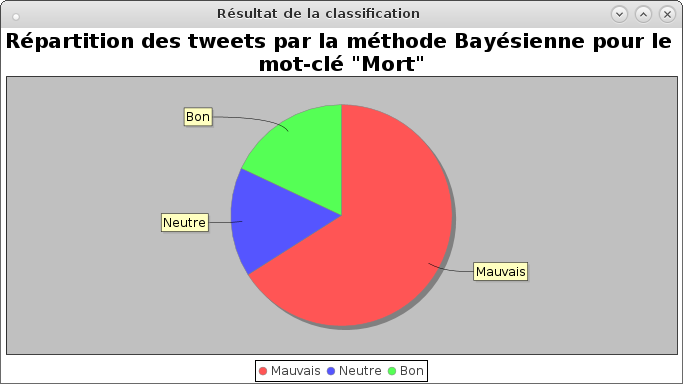
\includegraphics[width=0.45\textwidth]{img/classificationMortBayesTouslesMots.png}
	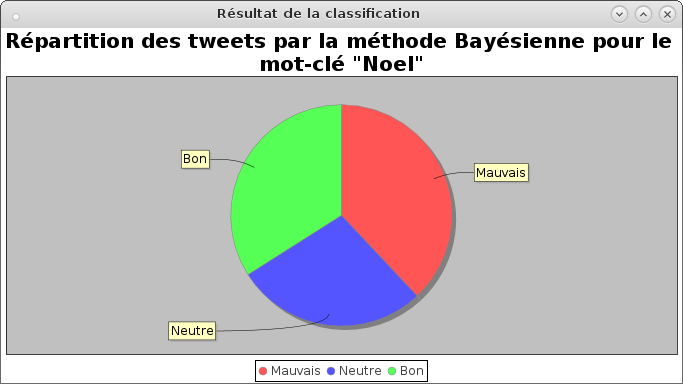
\includegraphics[width=0.45\textwidth]{img/classificationtouslesmotsnoel.png}
	\caption{Classification en prenant en compte tous les mots pour
	\textit{mort} (à gauche)\\et pour \textit{Noël} (à droite)}
	\label{bayes_tous_les_mots}
\end{figure}

\begin{figure}
	\centering
	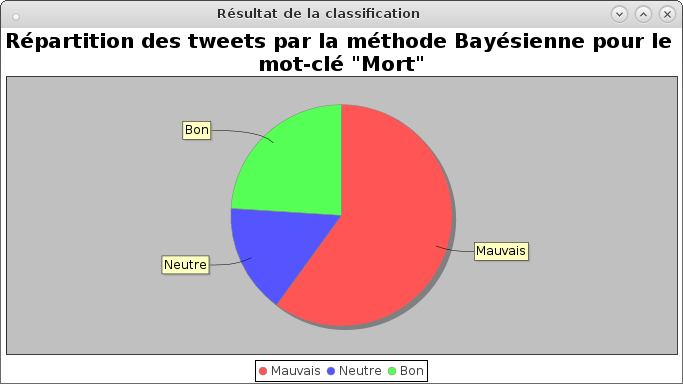
\includegraphics[width=0.45\textwidth]{img/classificationMortpastouslesMots.png}
	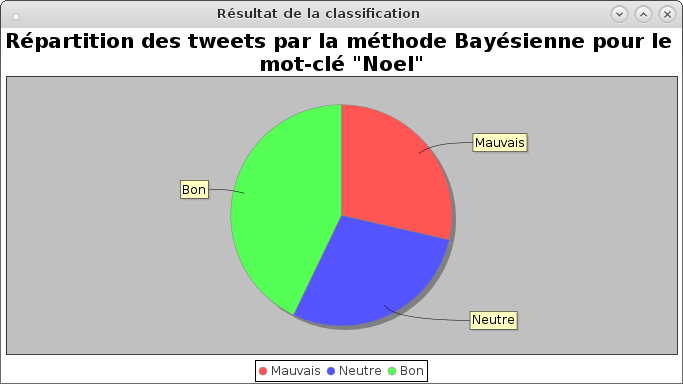
\includegraphics[width=0.45\textwidth]{img/classificationpastouslesmotsnoel.png}
	\caption{Classification sans tenir compte des mots courts pour
	\textit{mort} (à gauche)\\et pour \textit{Noël} (à droite)}
	\label{bayes_pas_tous_les_mots}
\end{figure}

Concernant la variante « fréquence » de la classification bayésienne, la
différence réside dans le fait que la probabilité qu'un mot appartienne à une
classe particulière est multiplié par le nombre de fois où le mot apparaît dans
le Tweet.

\subsection{Observations}
La méthode de classification bayésienne est en général une bonne méthode
d'annotation et elle ne dépend que d'un seul paramètre : la base de données de
Tweet (dans notre cas), contrairement à KNN qui dépend de $k$ et de la base de
données ou de la méthode par mot-clés qui ne dépend pas de la base, mais de deux
listes de mots arbitraires.

Cependant, au cours de nos tests, nous avons pu constater quelques faiblesses
pour cette méthode.

Comme on peut le voir sur la figure~\ref{capture_repartition_Tweetsv7}
(page~\pageref{capture_repartition_Tweetsv7}), cette
base n'est pas équilibrée, puisqu'elle comporte trop de Tweets « bons » par
rapport aux autres classes.

\begin{figure}
	\centering
	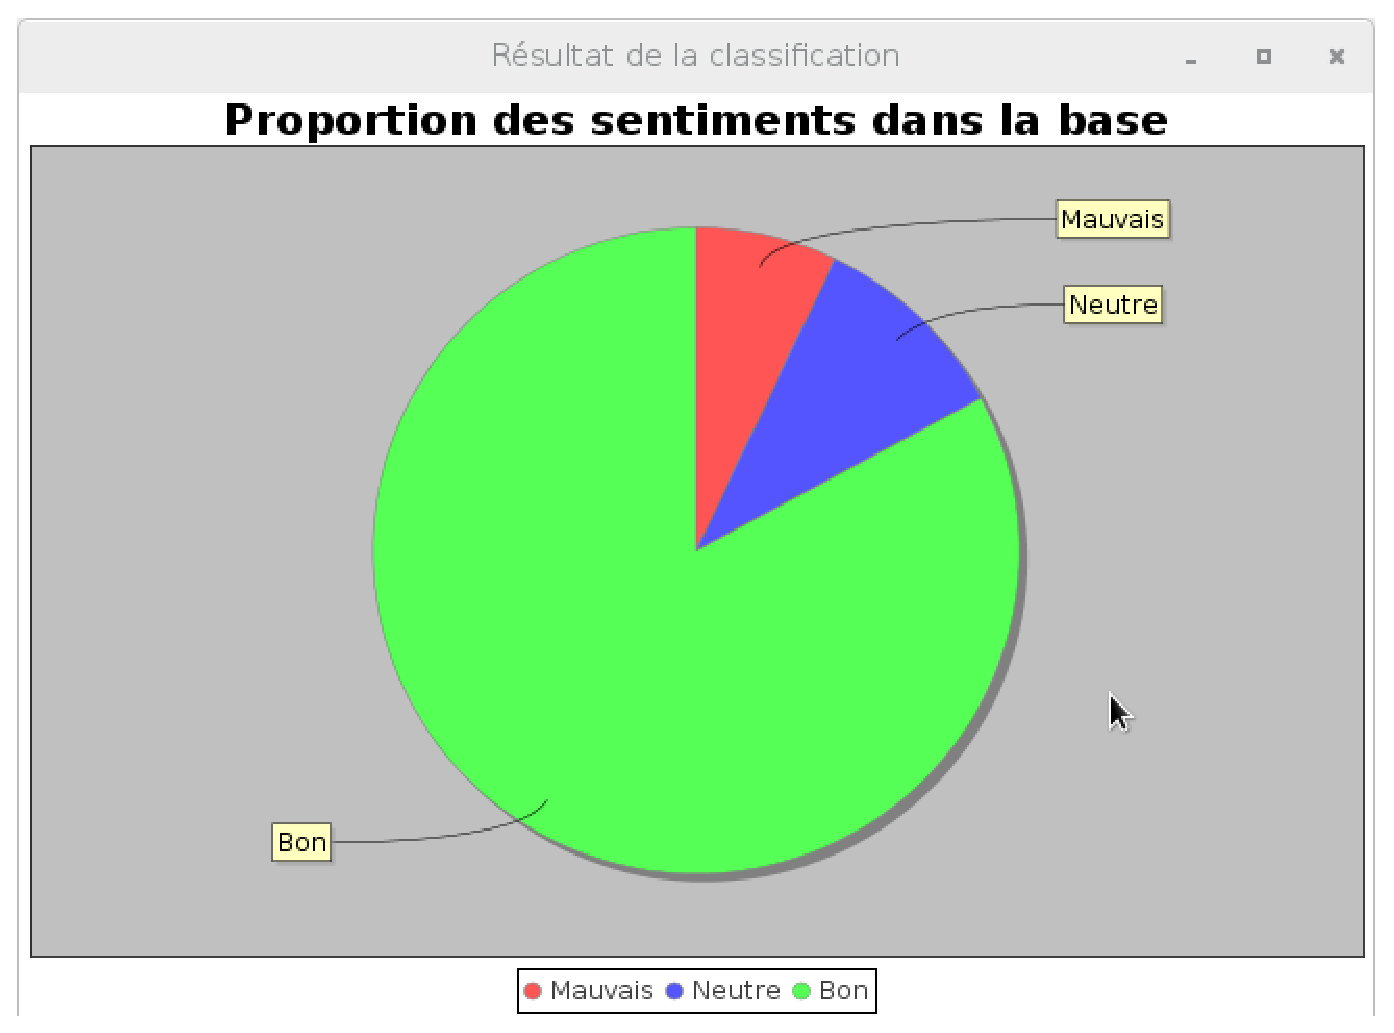
\includegraphics[width=0.45\textwidth]{img/resultats_classification_tweetsv7.eps}
	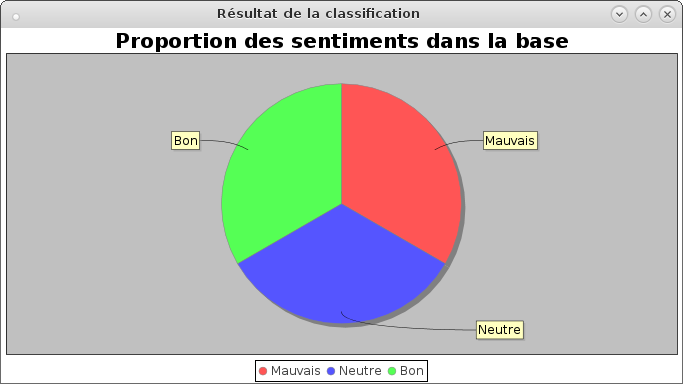
\includegraphics[width=0.45\textwidth]{img/classificationV8.png}
	\caption{Répartition des Tweets dans une de nos bases de données avant
	et après rééquilibrage.}
\label{capture_repartition_Tweetsv7}
\end{figure}

Ainsi, pour le mot-clé « mort », on obtient les résultats représentés par la
figure~\ref{capture_classification_mort_Tweetsv7}
(page~\pageref{capture_classification_mort_Tweetsv7}).

\begin{figure}
	\centering
	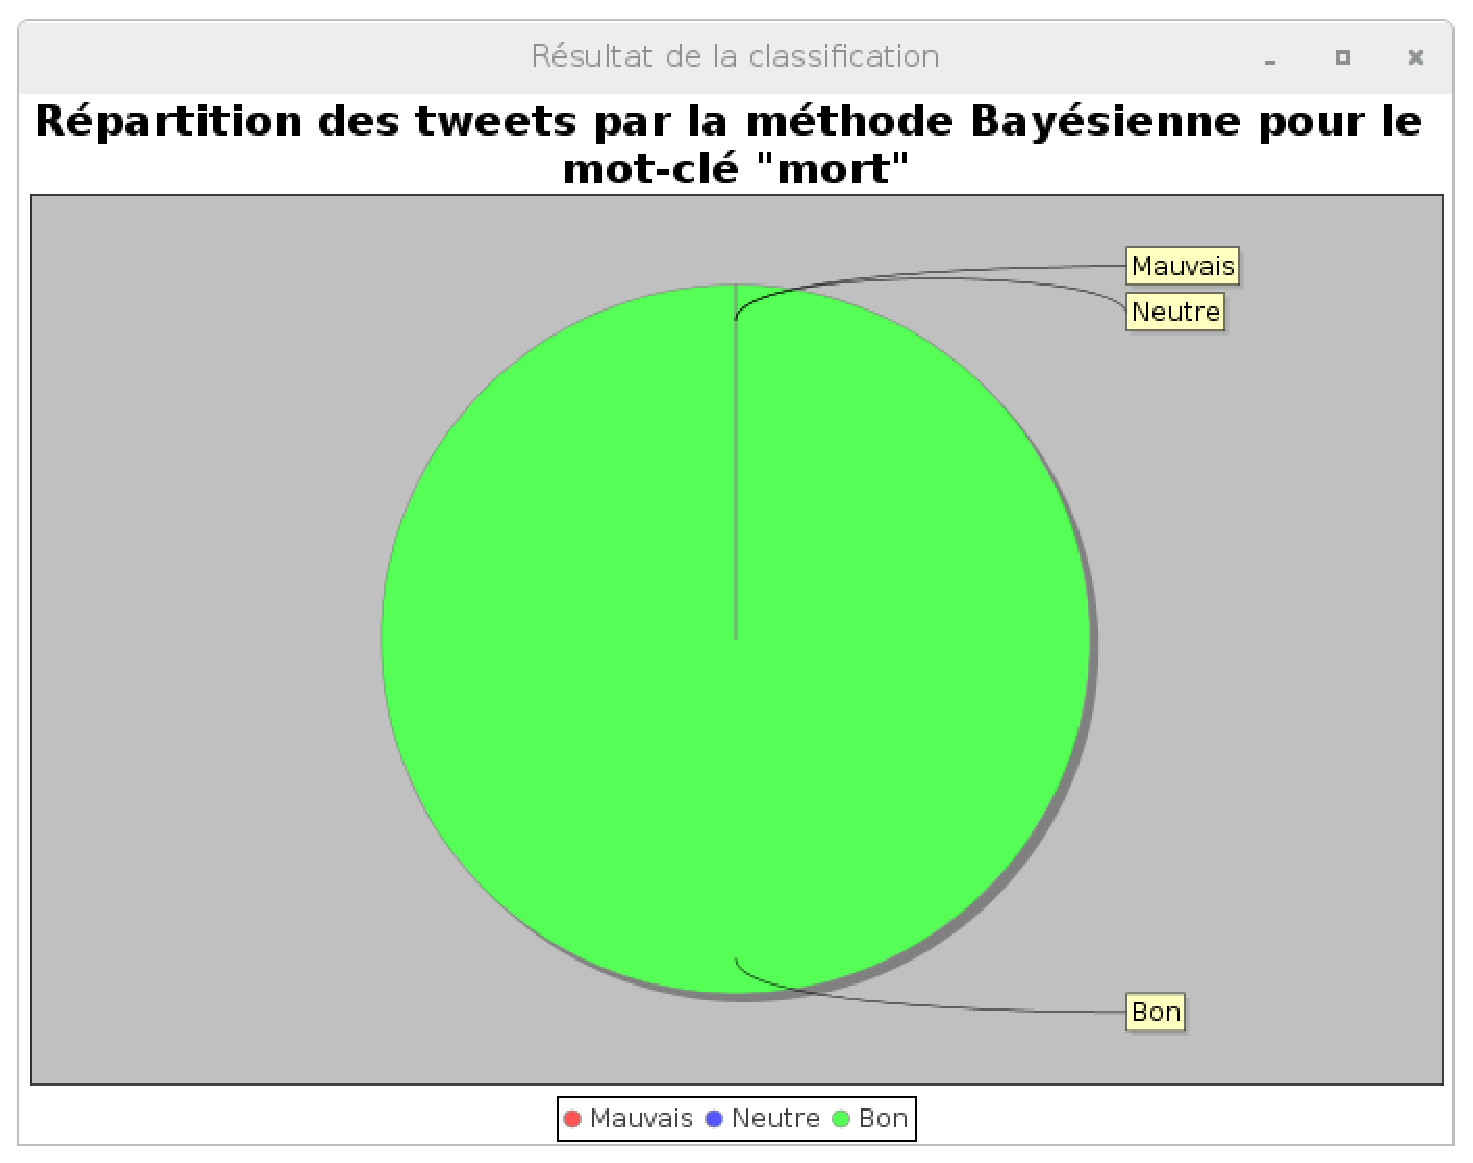
\includegraphics[width=0.45\textwidth]{img/bayes_annotation_mort_tweetsv7.eps}
	\caption{Annotation automatique pour le mot-clé « mort »}
\label{capture_classification_mort_Tweetsv7}
\end{figure}

On pourrait très bien penser que le mot « mort » n'a pas forcément une
connotation négative, prenons l'expression « Mort de rire ». Toutefois, le fait
que algorithme retourne 100\% de bon est clairement un problème.

Cela s'explique par le fait que la proportion de Tweets bon dans la base est
trop grande, ainsi la probabilité qu'un mot soit « Bon » est affecté
proportionnellement.

% -----------------------------------------------------------------------------

\chapter{Conclusion}
Ce projet était très intéressant sur plusieurs niveaux. Tout d'abord, il nous a
montré comment il était possible de connaître l'humeur d'une personne à partir
d'un simple message sur Twitter, mais aussi les difficultés qui en découlent.

Ces difficultés sont de deux types. Le premier, peut-être le plus évident, est
lié directement au format de Twitter, et plus particulièrement de sa limite des
cent quarante caractères, qui oblige parfois les utilisateurs à abréger ou à
supprimer des mots, voire à écrire dans une orthographe proche du langage SMS,
ce qui peut provoquer des faiblesses dans certains algorithmes. De plus,
certains éléments, typiquement la ponctuation, les \texttt{@usernames} et les
hashtags, provoquent du bruit dans mes Tweets et nécessitaient un nettoyage.
Une autre difficulté provenait de la base de données: pour avoir des résultats
cohérents, nous nous sommes rendus compte de m'importance de la répartition
générale des différentes classes. Ainsi, nous avons eu des difficultés lorsque
nous avons fusionné notre base de données avec celle d'un autre binôme, obtenant
une base de plus de mille Tweets contenant plus de 80\% de Tweets positifs,
comme nous l'avons mentionné dans le chapitre~\ref{classification_bayesienne}.

\CMName{} est donc l'aboutissement de beaucoup d'heures de travail qui nous ont
permis de connaître un nouveau moyen d'utiliser Twitter, de connaître des
algorithmes de classification et de savoir prendre du recul concernant les
résultats.

\end{document}
